\FloatBarrier
\section{Counterfactual Analysis}

Section 3.4 promised that a structure surviving Stage 3 licenses the third rung of the ladder, and this section redeems that promise on the fitted model. Three queries are evaluated. The first converts the posterior trend $\beta_T$ into a calendar-year decarbonisation rate and measures it against policy targets (Section 7.1). The second and third are the counterfactual queries of Section 3.4: what each building's compliance standing would be were the panel observed in 2030 (Section 7.2), and what each building would emit had it been built in 2010 (Section 7.3).

Every number in this section is an analytical function of the saved M6 posterior: each query substitutes one feature value in the linear predictor of Section 5.4, holds all other covariates at their observed values, and re-evaluates across the 12,000 draws and 21,406 compliant records, with no new sampling. The object being manipulated is the fitted predictor

\[
\mu_i = \alpha_{j[i]} + \beta_A \tilde{a}_i + \beta_B \tilde{b}_i + \beta_T \tilde{t}_i + \beta_Y \tilde{y}_i,
\]

in the notation of Section 5.4, evaluated at each posterior draw. Because the predictor is linear, substituting one feature moves each record's log-scale prediction by exactly one coefficient times the feature's displacement, which is why every query in this section reduces to one matrix operation per draw. Both intervened features sit outside the gate, which keys on floor area and property type alone, so the interventions leave each unit's compliance untouched; this is the action step of Section 3.4, and the queries concern the world layer alone.

\subsection{Decarbonisation Pace against Policy Benchmarks}

The posterior trend becomes a policy-readable rate once the standardisation is undone. $\beta_T$ measures the log-change per standard deviation of the data year, and one calendar year is $1/s_t$ of that unit, with $s_t = 2.590$ the panel's year standard deviation. The per-year rate is therefore

\[
r = \frac{\beta_T}{s_t} = \frac{-0.1447}{2.590} = -0.0559 \text{ log units per year},
\]

which exponentiates to $e^r - 1 = -5.43$ percent per year; applying the same map to every posterior draw gives the 89\% credible interval $[-5.61, -5.26]$ percent. This is the same parameter Section 6.2 reported on the standardised scale; the conversion changes its units, not its evidence.

The estimated pace clears the city's official target. A sustained rate $r$ reaches a fraction $q$ of the baseline after $\ln(q)/r$ years; equivalently, reaching fraction $q$ in $n$ years requires a rate of $\ln(q)/n$. The 2022 Chicago Climate Action Plan commits the city to a 62 percent reduction in citywide emissions by 2040 against a 2017 baseline (\cit{city2022}{City of Chicago, 2022}), which over that 23-year window requires $\ln(0.38)/23 = -0.0421$ log units per year. The estimated rate of $-0.0559$ exceeds it: sustained from 2017 to 2040, the trend delivers $1 - e^{23r} \approx 72$ percent. The comparison is indicative rather than conclusive, since the plan's target covers all sectors while the estimate describes the benchmarked building stock alone.

Full decarbonisation is a different matter, and a stricter benchmark shows where the trend alone gives out. At the estimated rate, an 80 percent reduction ($q = 0.20$) from the 2023 level takes $\ln(0.20)/(-0.0559) \approx 29$ years, arriving around 2052. A stylised net-zero-by-2040 benchmark, operationalised as a 99 percent reduction since the multiplicative scale cannot express zero, requires $r^\star = \ln(0.01)/17 = -0.2709$ log units per year over the seventeen years from 2023. That is $-23.73$ percent per year, roughly 4.4 times the estimated pace, leaving a shortfall of $r^\star - r = -0.2150$ log units per year (Figure 7.1). The comparison is between rates of change, not levels: the estimated rate is identified from the panel structure of the data, and the required rate follows from the target and the horizon, so the gap measures how far the observed dynamics are from the dynamics the target presumes.

Two qualifications bound the finding. The projection assumes the estimated trend persists unchanged to 2040, and the trend itself bundles the fall in the grid emission factor (Section 4.4) with efficiency change in the stock, so it is not a building-efficiency rate alone. Within those limits the rate is the best-defended number in the posterior: Section 6.5 found $\beta_T$ identical to three decimal places under every prior and weighting specification tested.

\begin{figure}[tbp]
\centering
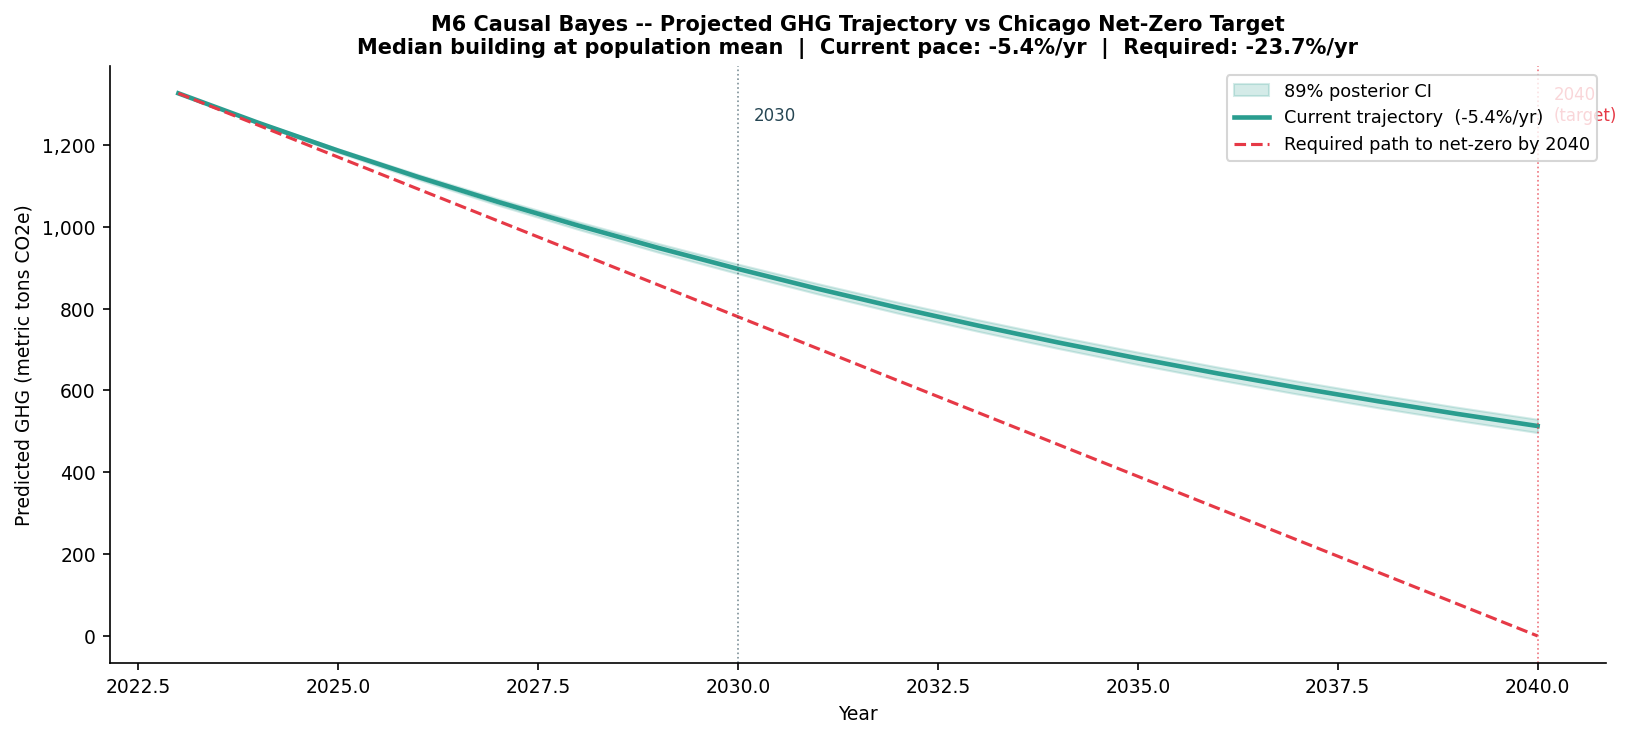
\includegraphics[width=0.95\linewidth]{figures/fig_trend.png}
\caption*{\textbf{Figure 7.1. Projected GHG trajectory against the stylised 2040 net-zero benchmark.} Posterior trajectory for a building at the population mean of the covariates, projected from 2023 at the estimated rate of $-5.4$ percent per year with its 89\% credible band, against the path required for full decarbonisation by 2040; the benchmark is stricter than the city's official 62 percent target (see text). Author's analysis of Chicago Energy Benchmarking data.}
\end{figure}

\subsection{Counterfactual 1: Compliance Risk in 2030}

The first counterfactual asks which buildings the trend alone will carry below a compliance threshold by 2030. The query sets the data year to 2030 for every record while holding size, type, vintage, and building count at observed values: the counterfactual year standardises to $\tilde{t}^\star = (2030 - 2019.1)/s_t = 4.21$, and replacing $\tilde{t}_i$ in $\mu_i$ shifts each record's log-scale prediction by $\beta_T(\tilde{t}^\star - \tilde{t}_i)$. The counterfactual year lies seven years past the panel's edge, so the query inherits the trend-persistence qualification of Section 7.1. For each posterior draw the residual is then added and the outcome back-transformed, $y^\star_i \sim \text{Normal}(\mu^\star_i, \sigma)$ with $\text{GHG}^\star_i = e^{y^\star_i} - 1$, and the compliance probability is the fraction of draws falling at or below the threshold $\tau$:

\[
P_i = P\big(\text{GHG}_i \leq \tau \mid do(\text{data year} = 2030)\big) = \frac{1}{12{,}000} \sum_{d=1}^{12{,}000} \mathbf{1}\{\text{GHG}^\star_{i,d} \leq \tau\}.
\]

Because the draws span the parameter posterior and the residual scale $\sigma$ jointly, $P_i$ carries both parameter uncertainty and building-level idiosyncrasy, and compliance becomes a probability rather than a verdict.

The threshold and the bands are stylised inputs, chosen for illustration rather than drawn from the ordinance. The threshold $\tau = 546$ metric tons CO$_2$e is the 25th percentile of observed GHG in the compliant training set, standing in for a performance standard; records are classified on-track when $P_i > 0.80$, high-risk when $P_i < 0.20$, and uncertain between. The contribution is the machinery, which applies unchanged to whatever threshold a regulator specifies.

Table 7.1 shows the portfolio splitting into three comparable blocks. The trend alone carries 35.4 percent of records on-track, leaves 37.1 percent at high risk even by 2030, and places 27.5 percent in the uncertain band; the median compliance probability across all records is 0.526, barely better than even odds. The uncertain band is the policy-relevant population, since these are the marginal cases where a targeted intervention could change the classification, while the high-risk block will not reach the threshold on trend continuation alone. The shares are over building-year records rather than buildings, so a building weighs in proportion to its reporting tenure.

\par\medskip\noindent
{\small\itshape \textbf{Table 7.1. Compliance classification under the 2030 counterfactual.} Records classified by posterior probability of falling below the 546 t CO$_2$e threshold when the data year is set to 2030. Author's analysis of Chicago Energy Benchmarking data.\par}
\nopagebreak\medskip\nopagebreak
{
\setlength{\tabcolsep}{7pt}
\renewcommand{\arraystretch}{1.15}
\begin{longtable}{lrrr}
\toprule
Classification & Criterion & Records & Share \\
\midrule
\endfirsthead
\toprule
Classification & Criterion & Records & Share \\
\midrule
\endhead
\bottomrule
\endlastfoot
On-track & $P_i > 0.80$ & 7,586 & 35.4\% \\
Uncertain & $0.20 \leq P_i \leq 0.80$ & 5,887 & 27.5\% \\
High-risk & $P_i < 0.20$ & 7,933 & 37.1\% \\
\end{longtable}
}
\par\medskip

This per-record probability is an output the point-prediction pipelines of Section 5 do not deliver. A point prediction combined with a hard threshold returns a single binary verdict per record; the posterior returns a probability, which is what risk-ranked targeting requires and what separates the marginal records from the firmly off-track ones.

\begin{figure}[H]
\centering
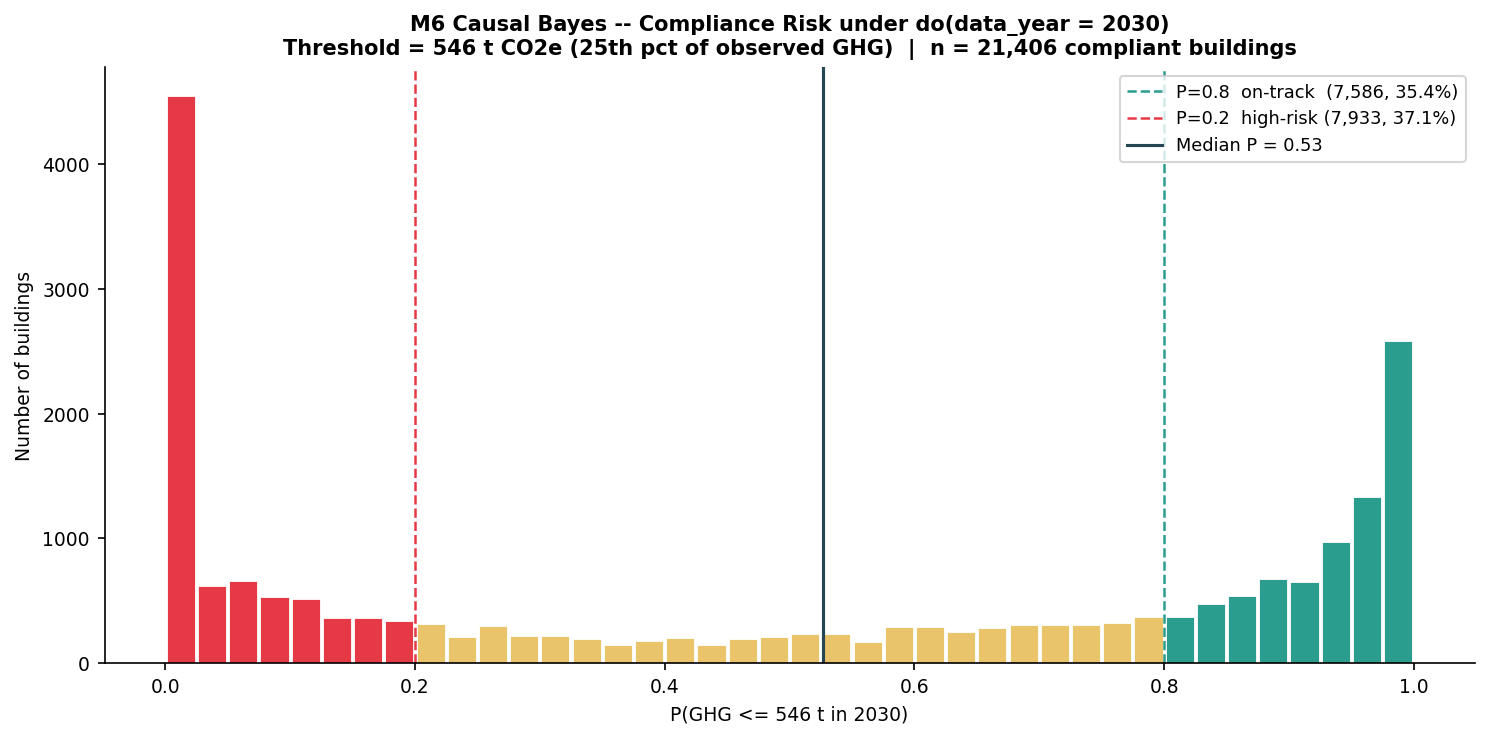
\includegraphics[width=0.95\linewidth]{figures/fig_cf1_compliance.png}
\caption*{\textbf{Figure 7.2. Compliance risk under the 2030 counterfactual.} Distribution of $P(\text{GHG} \leq 546\ \text{t})$ across the 21,406 compliant records with the 0.20 and 0.80 classification bounds and the median probability marked. Author's analysis of Chicago Energy Benchmarking data.}
\end{figure}

\subsection{Counterfactual 2: Vintage Reassignment}

The second counterfactual reassigns every building's construction year to 2010, against an actual mean vintage of 1964, and compares each record's predicted emissions under the two regimes. The disturbance enters both regimes identically and cancels from the contrast on the log scale, so the comparison requires only the posterior over the equations; this is the three-step computation of Section 3.4 (\cit{pearl2009}{Pearl, 2009}; \cit{pearletal2016}{Pearl, Glymour \& Jewell, 2016, Ch. 4}) with the action falling on the vintage node. Linearity makes the contrast exact: the factual and counterfactual predictors differ in the vintage term alone, so for each posterior draw

\[
\mu^{CF}_i - \mu^{F}_i = \beta_Y\,(\tilde{y}^\star - \tilde{y}_i) = \beta_Y \cdot \frac{2010 - v_i}{s_y}.
\]

Here $v_i$ is the record's actual construction year, $s_y = 37.4$ is the training-set standard deviation of year built, and $\tilde{y}^\star = (2010 - 1964.3)/s_y = 1.22$ is the counterfactual vintage on the training standardisation. The reported difference is taken on the original scale with the disturbance at its central value, $\Delta_i = (e^{\mu^F_i} - 1) - (e^{\mu^{CF}_i} - 1)$, and summarised per record across the 12,000 draws.

The result runs against the intuition that newer means cleaner. The median per-record difference, factual minus counterfactual, is $-48$ metric tons CO$_2$e, and the 89\% credible interval for a typical record is $[-53, -42]$: the 2010-vintage counterfactual is predicted to emit more, not less. The direction is near-uniform, with 90.2 percent of records showing a credible increase, 8.8 percent a credible reduction, and 1.0 percent no credible effect (Figure 7.3). The mean difference of $-115$ t exceeds the median because the deltas scale with building size. The magnitude follows directly from the Section 6.2 posterior: a building of mean vintage moves 1.22 standard deviations, which at $\beta_Y = 0.047$ shifts the log scale by $0.047 \times 1.22 \approx 0.057$ and multiplies predicted emissions by $e^{0.057} \approx 1.06$; six percent of a median-sized building is some 50 to 60 t, consistent with the reported median.

The sign is counterintuitive only if $\beta_Y$ is read as a building-code efficiency effect, which the tested structure says it is not. The DAG carries reporting year and construction year on separate nodes, and Section 6.2 showed the posterior separating them: $\beta_T$ absorbs the year-on-year efficiency improvement, so what remains in $\beta_Y$ is the cross-sectional composition of vintage cohorts, consistent with the reading given there that newer construction in the benchmarked stock houses more energy-intensive operations. Under that reading, reassigning a 1960s building to 2010 moves it into a more intensive cohort, and the model predicts higher emissions accordingly.

Two implications follow, one for policy and one for method. For policy, vintage is a poorly targeted instrument: a programme that rewards newer construction as such would reward the more intensive cohort, and area-normalised intensity standards by property type are the better-aimed lever. For method, this query is not a retrofit-impact estimator and should not be read as one, because a retrofit operates through the energy mediators, which are compliance-gated and outside the upstream feature set; estimating that effect requires the mediator layer and is beyond this paper's scope.

\begin{figure}[H]
\centering
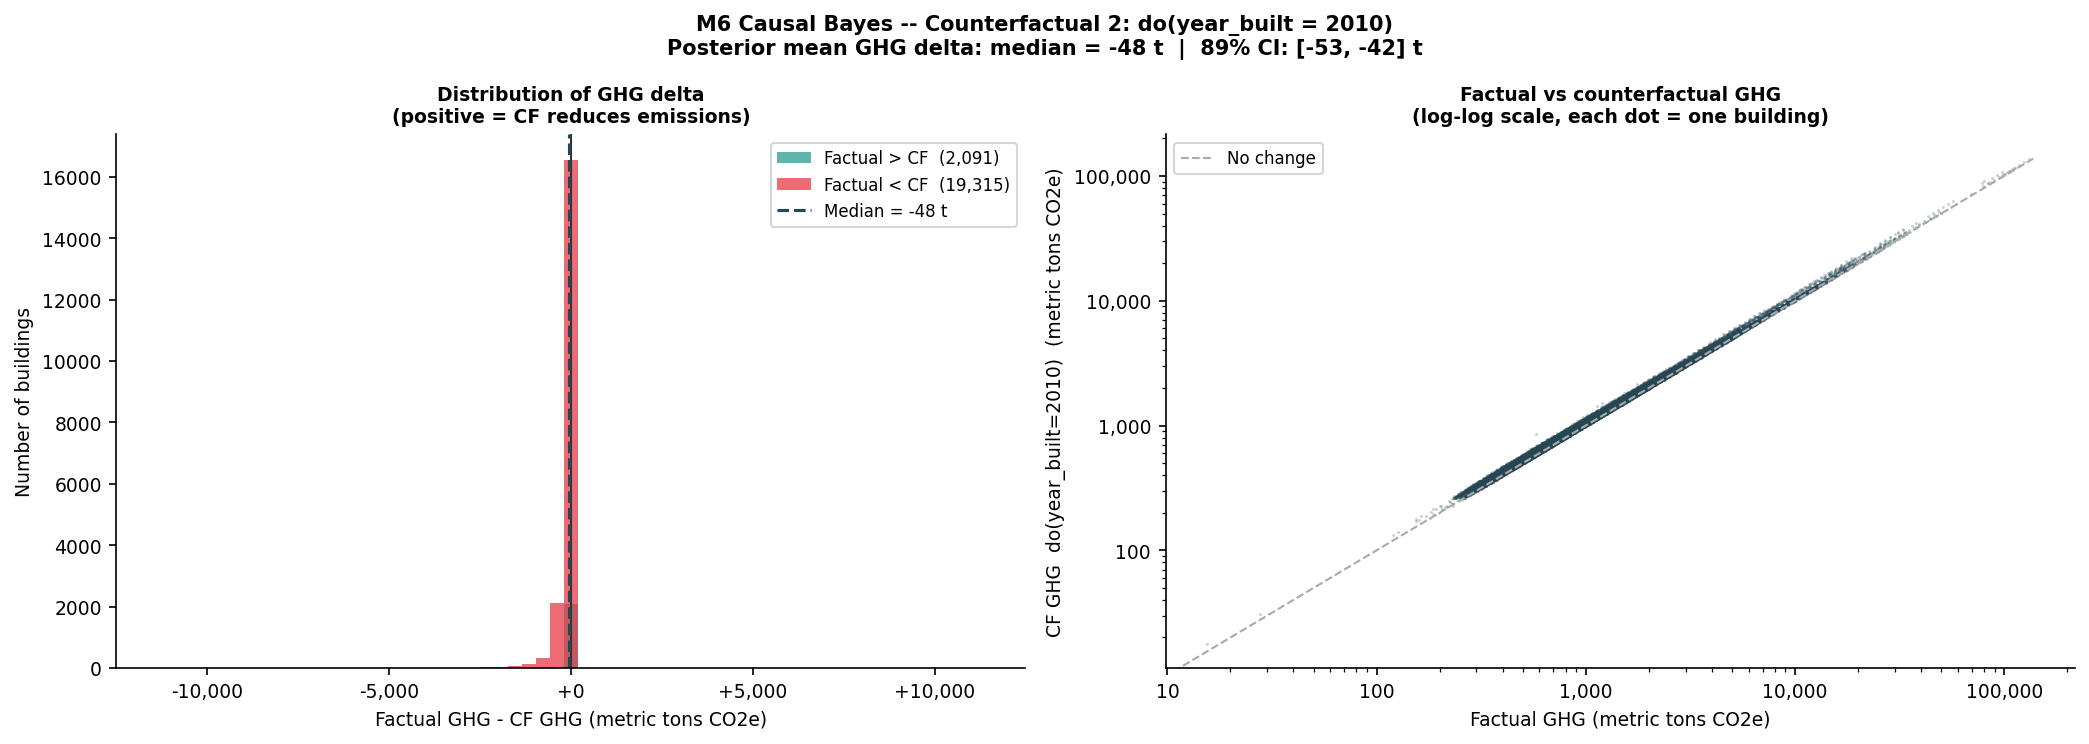
\includegraphics[width=0.95\linewidth]{figures/fig_cf2_reduction.png}
\caption*{\textbf{Figure 7.3. Vintage reassignment counterfactual.} Left: distribution of the per-record mean difference $\Delta_i$ under the 2010 reassignment, with the median marked; negative values mean the counterfactual vintage is predicted to emit more. Right: factual against counterfactual predicted GHG per record on log-log axes, where points below the diagonal would indicate a reduction. Author's analysis of Chicago Energy Benchmarking data.}
\end{figure}

The two counterfactual queries close the ladder the paper set out to climb: seeing in the shadow matrix and the associational models, doing in the inverse-probability correction, imagining in the counterfactuals of this section (\cit{pearl2009}{Pearl, 2009}). The vintage query is the sharper demonstration of why the climb matters. Its computation would have been equally possible on an asserted graph, but its counterintuitive answer would then have been indistinguishable from a specification artefact; on the tested structure, the answer has a warrant, because the separation of trend from cohort that produces it is carried by the structure that survived Stage 3.

